\section{Experiments}
\label{sec:experiments}

We evaluate \texttt{semflow-dl} on both a controlled nonlinear causal mediation benchmark with known counterfactual ground truth and a large-scale wind-turbine SCADA engineering case study. All experiments were executed in isolated subprocesses on an Intel MacBook Pro (2017, 8~GB RAM, CPU-only), measuring wall-clock median latency and true peak resident set size (RSS) via POSIX \texttt{wait4}.

\subsection{Nonlinear Causal Mediation vs.\ EBM and XGBoost+SHAP}
To isolate mediator blocking, measurement attenuation, and tail monotonicity violations, we construct a structural causal dataset ($N \in \{10^4, 10^5\}$, split 70\%/15\%/15\% into Train/Cal/Test) with three anchored latents (\texttt{Load}, \texttt{Stress}, \texttt{Risk}, two noisy indicators each, $\lambda \in [0.85, 0.92]$):
\begin{align*}
  \mathrm{Stress}_{\mathrm{raw}} &= 1.15\tanh(0.85\,\mathrm{Load}) + 0.25\,\mathrm{Load} + 0.45\,\varepsilon_S, \\
  \mathrm{Risk}_{\mathrm{raw}}   &= 0.65\ln(1 + e^{1.25\,\mathrm{Stress}_{\mathrm{std}}}) + 0.14\,\mathrm{Load} + 0.40\,\varepsilon_Y,
\end{align*}
where $\approx 73\%$ of the total causal effect of $\mathrm{do}(\mathrm{Load} + 1\,\mathrm{SD})$ flows indirectly through \texttt{Stress}. We compare \texttt{semflow-dl} (order-3 monotonic I-Splines, 6 quantile knots, 95\% split-conformal calibration) against a linear-edge ablation (\texttt{semflow-linear}), a 1D Explainable Boosting Machine (\texttt{EBM}) \citep{lou2013accurate}, and \texttt{XGBoost} \citep{chen2016xgboost} with \texttt{TreeSHAP} \citep{lundberg2017unified}.

\begin{table}[t]
  \centering
  \caption{Quantitative comparison on nonlinear causal mediation ($N = 10{,}000$ and $100{,}000$). \texttt{semflow-dl} reduces $\mathrm{do}(\mathrm{Load} + 1\,\mathrm{SD})$ error by $>5\times$, guarantees $0.0\%$ monotonicity violations, explains/intervenes $87.6\times$ faster than \texttt{XGBoost+SHAP} at $10$K ($8.6\times$ at $100$K), and uses $2.4\times\text{--}2.9\times$ less RAM.}
  \label{tab:whitebox-bench}
  \resizebox{\textwidth}{!}{%
  \small
  \begin{tabular}{rlrrrrrrrr}
    \hline
    $N$ & Engine & $R^2_{\mathrm{Oracle}}$ & $|\Delta \mathrm{do}|$ Err & Indirect Est & Load Credit & Mono Viol & Fit (ms) & Exp (ms) & Peak RSS \\
    \hline
    10K  & \texttt{semflow-dl}     & 0.5948 & \textbf{0.0816} & $+0.3678$ & 58.0\% & \textbf{0.0\%} & 246.04  & 12.56   & \textbf{58.11 MB} \\
    10K  & \texttt{semflow-linear} & 0.5731 & 0.1221          & $+0.3521$ & 58.7\% & 0.0\%          & 3.00    & 0.97    & 56.75 MB \\
    10K  & \texttt{ebm}            & 0.5957 & 0.4719          & $0.0000$  & 38.5\% & 1.0\%          & 1653.08 & 4.17    & 182.27 MB \\
    10K  & \texttt{xgb\_shap}      & 0.5658 & 0.4735          & $0.0000$  & 33.5\% & 33.2\%         & 462.25  & 1099.88 & 236.85 MB \\
    \hline
    100K & \texttt{semflow-dl}     & 0.5767 & \textbf{0.0942} & $+0.3732$ & 63.5\% & \textbf{0.0\%} & 5898.00 & 163.32  & \textbf{86.83 MB} \\
    100K & \texttt{semflow-linear} & 0.5553 & 0.1346          & $+0.3591$ & 58.0\% & 0.0\%          & 37.92   & 7.40    & 68.85 MB \\
    100K & \texttt{ebm}            & 0.5776 & 0.4927          & $0.0000$  & 36.6\% & 5.0\%          & 12673.49& 11.14   & 206.02 MB \\
    100K & \texttt{xgb\_shap}      & 0.5762 & 0.5172          & $0.0000$  & 29.6\% & 25.6\%         & 1830.38 & 1411.57 & 247.79 MB \\
    \hline
  \end{tabular}%
  }
\end{table}

As shown in Table~\ref{tab:whitebox-bench}, flat predictors (\texttt{EBM} and \texttt{XGBoost+SHAP}) suffer severe mediator blocking ($\mathrm{AIE}_{\mathrm{Indirect}} \equiv 0$), underestimating $\mathrm{do}(\mathrm{Load}+1\,\mathrm{SD})$ by $0.4719\text{--}0.5172$ SD and exhibiting $1.0\%\text{--}33.2\%$ monotonicity violations in sparsely populated tails. By contrast, \texttt{semflow-dl} recovers both the saturating \texttt{Load}$\to$\texttt{Stress} curve and convex \texttt{Stress}$\to$\texttt{Risk} acceleration with exact M-Spline local elasticity $\phi'(z)$, $0.0\%$ monotonicity violations, and $5\times$ lower intervention error.

\begin{figure*}[t]
  \centering
  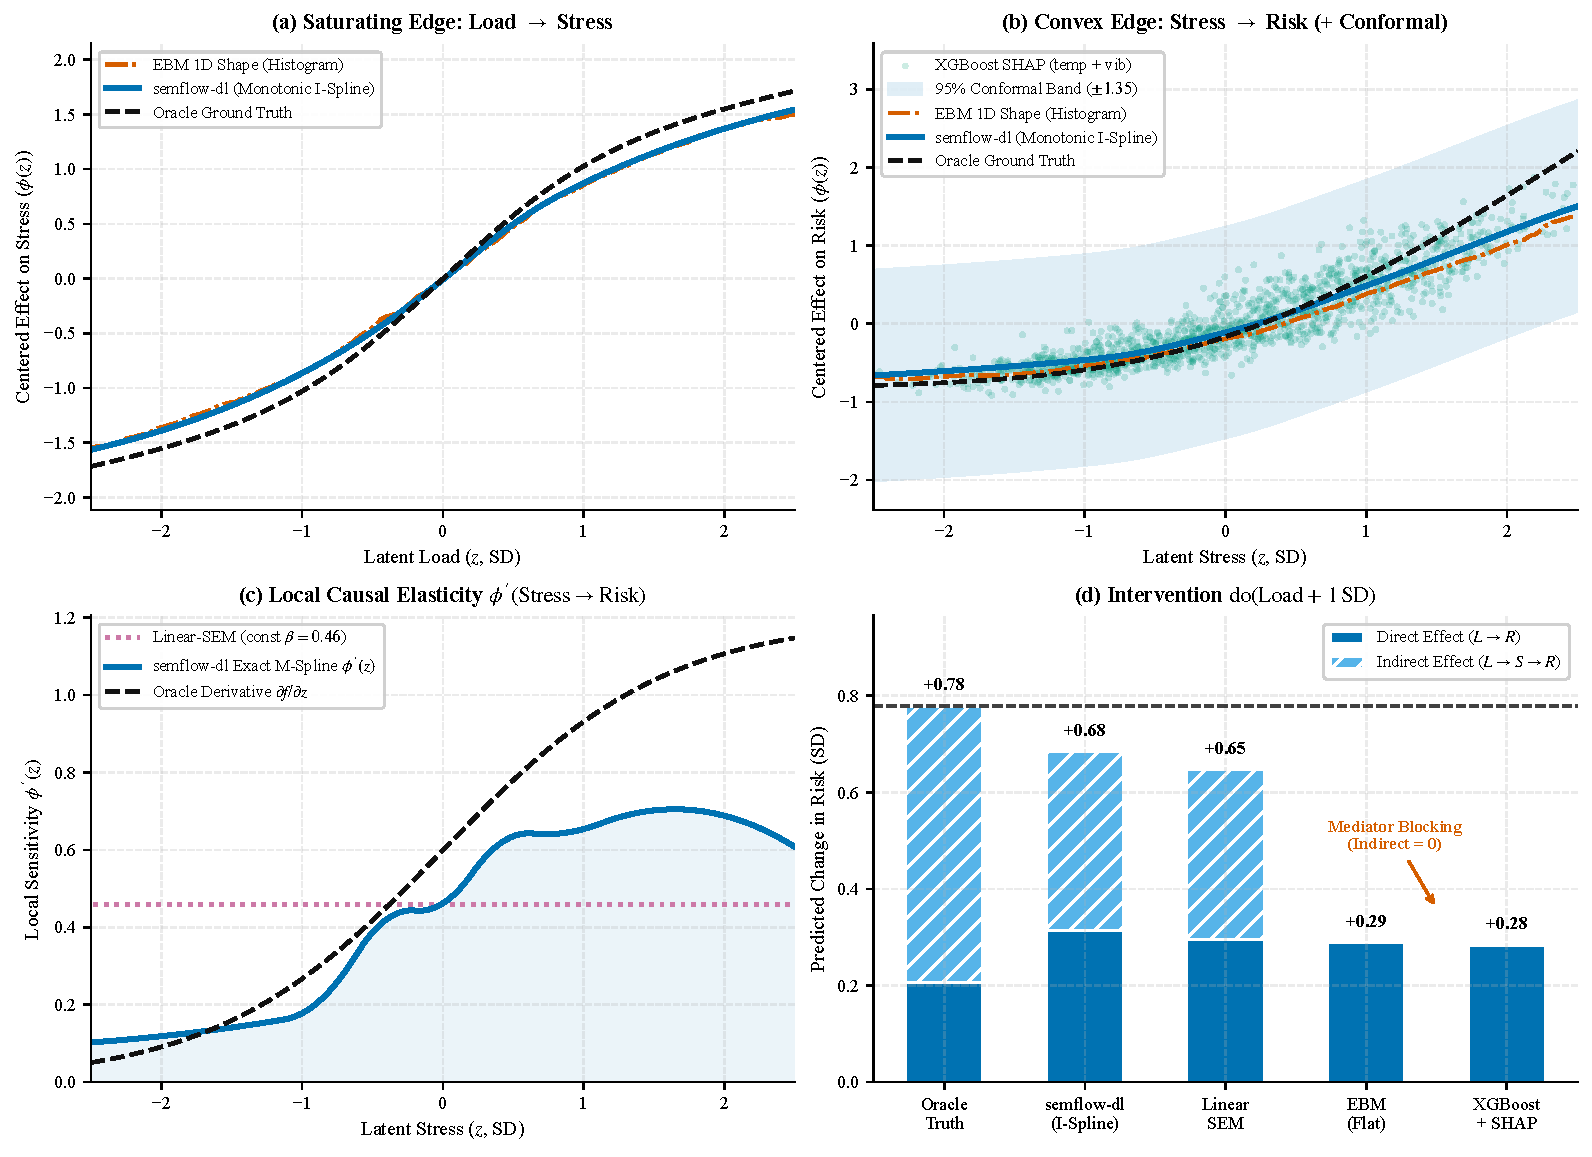
\includegraphics[width=\textwidth]{figures/fig_whitebox_4panel.pdf}
  \caption{Qualitative and causal comparison on the nonlinear mediation benchmark ($\mathrm{Load} \to \mathrm{Stress} \to \mathrm{Risk}$ with noisy dual indicators).
  \textbf{(a)}~Saturating edge recovery ($\mathrm{Load} \to \mathrm{Stress}$): \texttt{semflow-dl} tracks the monotonic ground truth smoothly without histogram binning artifacts.
  \textbf{(b)}~Convex edge recovery ($\mathrm{Stress} \to \mathrm{Risk}$) with 95\% split-conformal prediction bands ($\pm 1.35$\,SD), contrasted against dispersed TreeSHAP attributions and EBM step curves.
  \textbf{(c)}~Closed-form local causal elasticity $\phi'(\mathrm{Stress} \to \mathrm{Risk})$ via M-Spline derivatives, capturing tail-risk acceleration missed by constant-slope Linear-SEM ($\beta = 0.46$).
  \textbf{(d)}~Structural intervention $\mathrm{do}(\mathrm{Load} + 1\,\mathrm{SD})$, illustrating severe mediator blocking ($\mathrm{Indirect} = 0$) in flat EBM and XGBoost+SHAP versus accurate direct--indirect decomposition in \texttt{semflow-dl}.}
  \label{fig:whitebox-4panel}
\end{figure*}

Figure~\ref{fig:whitebox-4panel} visually confirms these quantitative findings. In Panels~(a) and~(b), \texttt{semflow-dl} recovers both the saturating $\mathrm{Load} \to \mathrm{Stress}$ curve and the convex $\mathrm{Stress} \to \mathrm{Risk}$ acceleration smoothly across $[-2.5, +2.5]$\,SD while enclosing test observations within finite-sample 95\% split-conformal bands ($\pm 1.35$\,SD). Panel~(c) highlights a core advantage over both Linear-SEM and flat glass-box models: the exact M-Spline derivative $\phi'(z)$ reveals how marginal risk sensitivity rises from near-zero under low stress to over $0.70$ under high stress, whereas Linear-SEM collapses this regime shift into a single constant slope ($\beta = 0.46$). Finally, Panel~(d) demonstrates why flat models fail under policy simulation: because EBM and XGBoost+SHAP hold the noisy mediator indicators fixed during perturbation, their predicted intervention effects ($+0.29$ and $+0.28$\,SD) miss the entire indirect pathway, whereas \texttt{semflow-dl} ($+0.68$\,SD) closely recovers the oracle total effect ($+0.78$\,SD) and cleanly separates direct and indirect contributions.

\subsection{Wind Turbine SCADA Thermal Stress Case Study}
On a physics-grounded wind-turbine SCADA dataset ($N = 50{,}000$, with $2\%\text{--}4\%$ sensor dropout) modeling $\texttt{Wind} \to \texttt{Load} \to \texttt{Stress} \to \texttt{Loss}$, \texttt{semflow-dl} fits the entire DAG with 95\% split-conformal calibration in $5.0$~s (Table~\ref{tab:scada-case}), decomposing $\mathrm{do}(\mathrm{Load} + 1\,\mathrm{SD})$ on \texttt{Loss} into $+0.2824$ direct and $+0.1838$ indirect effects ($+0.4662$ total), while revealing a $5.6\times$ increase in local thermal elasticity $\phi'(\mathrm{Load} \to \texttt{Stress})$ from low load ($0.087$) to high load ($0.489$).

\begin{table}[t]
  \centering
  \caption{Wind-turbine SCADA thermal stress case study summary ($N = 50{,}000$, 2\%--4\% sensor dropout).}
  \label{tab:scada-case}
  \small
  \begin{tabular}{lll}
    \hline
    Metric / Causal Quantity & \texttt{semflow-dl} (I-Spline + Conformal) & Interpretation \\
    \hline
    Total Fit + Calibration Time & 5.00 s & CPU-only, 95\% Split-Conformal \\
    $\mathrm{do}(\mathrm{Load} + 1\,\mathrm{SD}) \to \mathrm{Loss}$ (Total) & $+0.4662$ SD & Direct $+0.2824$ + Indirect $+0.1838$ \\
    Local Elasticity $\phi'(\mathrm{Load} \to \mathrm{Stress})$ (Low Load) & $0.087$ & Mild thermal sensitivity \\
    Local Elasticity $\phi'(\mathrm{Load} \to \mathrm{Stress})$ (High Load) & $0.489$ & \textbf{5.6$\times$} thermal acceleration regime \\
    \hline
  \end{tabular}
\end{table}
